\documentclass[12pt,dvipsnames]{article}
\setcounter{section}{0}

\usepackage{amsmath,amsthm,amssymb,amsbsy}
\usepackage[spanish,es-tabla]{babel}
\decimalpoint
\usepackage{braket}
\usepackage{color}
\usepackage{enumitem}
\usepackage{fancyhdr}
\usepackage{float}
\usepackage[T1]{fontenc}
\usepackage[margin=1.5cm]{geometry} 
\usepackage{graphicx}
\graphicspath{ {images/} }
\usepackage{hyperref}
\usepackage[utf8]{inputenc}
\usepackage{listings}
\usepackage{lmodern}
\usepackage{multicol}
\usepackage{multirow}
\usepackage{pgfplots}
\usepackage{soul}
\usepackage{tabularx}
\usepackage{tcolorbox}
\tcbuselibrary{listings,breakable}
\usepackage{tikz}
\usetikzlibrary{babel}
\usepackage{url}
\usepackage{wrapfig}
\usepackage{xcolor}

\setlength{\parindent}{1em}
\setlength{\parskip}{1em}

\definecolor{NARANJA}{rgb}{1,0.467,0}
\definecolor{VERDE}{rgb}{0.31,1,0}
\definecolor{AZUL}{rgb}{0,0.53,1}
\definecolor{ROJO}{rgb}{1,0,0}

\hypersetup{
    colorlinks=true,
    linkcolor=ROJO,
    filecolor=magenta,      
    urlcolor=AZUL,
}
 
\pgfplotsset{compat=1.15}
 
\renewcommand{\figurename}{Figura}

\newcommand{\anim}[2]{\textcolor{red}{\textbf{\hl{#1}}}\footnote{#2}}

\renewcommand{\indexname}{Índice}
\renewcommand{\appendixname}{Apéndice}
\renewcommand{\contentsname}{Contenidos}
\renewcommand{\proofname}{Dem.}
\renewcommand{\tablename}{Tabla.}
\renewcommand\qedsymbol{$\blacksquare$}
\newtheorem{teo}{Teorema}[section]
\newtheorem{cor}{Corolario}[section]
\newtheorem{lem}{Lema}[section]
\newtheorem{defi}{Definición}[section]
\newtheorem{obs}{Observación}[section]
\newtheorem{prop}{Propiedades.}[section]
\newtheorem{ejem}{\textbf{\textit{$\circ \ \text{Ejemplo}$}}}[section]
\newtheorem{axi}{Axioma}[section]

\numberwithin{equation}{section}

%%%%%%%%%%%%%%%%%%%%%%%%%%%%%%%%%%%%%%%%%%%%%%%%%%%%%cajas

\newtcolorbox{post}{colback=white,colframe=red!50!black,
	colbacktitle=red!75!black, title= Postulado.}

\newtcolorbox{enu}{colframe=white!85!black, colback=white, leftrule = 10mm, sharp corners, breakable}

\newtcolorbox{solu}{colframe=black, colback=white, leftrule = 1mm, rightrule = -1mm,toprule = -1mm, bottomrule=-1mm, sharp corners, breakable}

\newtcolorbox{corre}{colframe=red, colback=white, leftrule = 1mm, rightrule = -1mm,toprule = -1mm, bottomrule=-1mm, sharp corners, breakable}

\newtcolorbox{enun}{colframe=gray, colback=white!90!black, leftrule = 1mm, rightrule = 1mm, toprule = -1mm, bottomrule=-1mm, sharp corners, breakable}

%%%%%%%%%%%%%%%%%%%%%%%%%%%%%%%%%%%%%%%%%%%%%%%%%%%%%cajas

%%%%%%%%%%%%%%%%%%%%%%%%%%%%%%%%%%%%%%%%%%%%%%%%%%%%%demarcado de soluciones

%New colors defined below
\definecolor{codegreen}{rgb}{0,0.6,0}
\definecolor{codegray}{rgb}{0.5,0.5,0.5}
\definecolor{codepurple}{rgb}{0.58,0,0.82}
\definecolor{backcolour}{rgb}{0.95,0.95,0.92}

%Code listing style named "mystyle"
\lstdefinestyle{mystyle}{
	backgroundcolor=\color{backcolour},   commentstyle=\color{codegreen},
	keywordstyle=\color{magenta},
	numberstyle=\tiny\color{codegray},
	stringstyle=\color{codepurple},
	basicstyle=\ttfamily\footnotesize,
	breakatwhitespace=false,         
	breaklines=true,                 
	captionpos=b,                    
	keepspaces=true,                 
	numbers=left,                    
	numbersep=5pt,                  
	showspaces=false,                
	showstringspaces=false,
	showtabs=false,                  
	tabsize=2
}

%"mystyle" code listing set
\lstset{style=mystyle}

\newenvironment{sol}{\begin{figure}[H]
		\begin{tikzpicture}
		\filldraw[black] (0,0) circle (3pt);
		\draw[line width = 0.5pt] (0,0) -- (4,0) node[above right]{\textbf{Solución:}};
		\end{tikzpicture}
\end{figure}}{\begin{figure}[H]
		\begin{flushright}
			\begin{tikzpicture}
			\draw[line width = 0.5pt] (0,0)-- (4,0);
			\filldraw (4,0) circle (3pt);
			\end{tikzpicture}
\end{flushright}\end{figure}}

%%%%%%%%%%%%%%%%%%%%%%%%%%%%%%%%%%%%%%%%%%%%%%%%%%%%%demarcado de soluciones
 
\begin{document}

\title{Ortogonalización y ortonormalización \\ (Proceso de Gram-Schmidt) \\ $(\approx 99\%)$}
\date{}
\maketitle
%\tableofcontents

\begin{obs}

Las ideas principales detrás del Teorema de Gram-Schmidt son tres:
\begin{enumerate}[label=(\roman*)]
    
    \item en espacios vectoriales de dimensión finita con producto escalar, los conjuntos l.i. se pueden ortogonalizar/ortonormalizar,
    
    \item el conjunto ortogonal/ortonormal obtenido a partir del conjunto l.i. genera al mismo subespacio vectorial que el conjunto l.i. y
    
    \item sigue siendo l.i.
\end{enumerate}

El objetivo es mostrar estas tres ideas geométricamente para generar la intuición necesaria para entender el teorema.
\end{obs}

\newpage
\section{Primera escena}

Supongamos que tenemos un plano con dos vectores linealmente independientes\footnote{Mostramos brevemente que están en ejes distintos.}, pero no ortogonales entre sí, y que queremos modificar alguno de ellos, utilizando las operaciones que ya conocemos\footnote{Mostramos brevemente algo como $\vec{u}+\vec{v}, a\vec{u}, \langle\vec{u},\vec{v}\rangle$ en pantalla, para que se entienda que nos referimos a las operaciones de suma vectorial, producto de un vector por un escalar y producto escalar.}, de tal forma que obtengamos un conjunto ortogonal\footnote{Mostramos $\Gamma_1=\{ \text{?`} ? \}$ en pantalla.} de dos vectores a partir de nuestro conjunto linealmente independiente\footnote{Resaltamos a $I=\{\vec{a},\vec{b}\}$.}, el cual genera a todo el plano\footnote{Mostramos que $\langle I\rangle$ es todo el plano.}.

Por definición, el hecho de que nuestros vectores no sean ortogonales significa que su producto escalar es distinto de cero\footnote{Mostramos $\langle \vec{a},\vec{b}\rangle\neq0$ en pantalla.}, por lo que la proyección vectorial\footnote{Hacemos dos proyecciones vectoriales rápidas para mostrar que, en efecto, son no nulas.} de cualquiera de ellos sobre el otro es distinta del vector nulo. Dicho de otra forma, ambos vectores deben tener una componente no nula a lo largo del eje del otro vector, por la propiedad\footnote{Debajo de $\langle\vec{a},\vec{b}\rangle\neq0$, mostramos brevemente $\langle \vec{b},\vec{a}\rangle = \overline{\langle \vec{a},\vec{b}\rangle}$ y, abajo, $\implies \langle\vec{b},\vec{a}\rangle\neq0$ (quedaría como un silogismo); luego, desaparecemos los tres renglones, junto con la proyección vectorial de $\vec{a}$ sobre $\vec{b}$.} de simetría conjugada del producto escalar.

¿Qué pasa si le removemos\footnote{Usamos la proyección vectorial de $\vec{b}$ sobre $\vec{a}$ para ortogonalizar a $\vec{b}$, obteniendo así a $\vec{b}'$, y escribimos $\Gamma_1=\{\vec{a},\vec{b}'\}$.} esta componente a uno de los vectores? Obtenemos un conjunto ortogonal, ¡como queríamos! Observemos que dicho conjunto ortogonal \emph{genera el mismo subespacio vectorial que el conjunto linealmente independiente con el que empezamos}\footnote{Mostramos al generado de $\Gamma_1$ (que es todo el plano) y escribimos $\langle \Gamma_1 \rangle = \langle I \rangle$ en pantalla.}; esto se debe a que obtuvimos al vector $\vec{b}'$ como combinación lineal de los vectores de $I$ y, además, a que los vectores claramente no perdieron su independencia lineal\footnote{Trazamos líneas punteadas para mostrar que los vectores ortogonalizados están ejes distintos.} cuando los ortogonalizamos.

Por otro lado\footnote{Regresamos al conjunto $I$ original con las dos proyecciones vectoriales, desaparecemos ahora a la proyección vectorial de $\vec{b}$ sobre $\vec{a}$ y usamos la de $\vec{a}$ sobre $\vec{b}$ para ortogonalizar a $\vec{a}$ y obtener así a $\vec{a}'$.}, si, partiendo de nuestro conjunto original, hubiéramos decidido modificar al \emph{otro} vector, hubiéramos obtenido un conjunto ortogonal \emph{distinto}\footnote{Escribimos $\Gamma_2=\{\vec{a}',\vec{b}\}$ en pantalla.} al anterior pero que, nuevamente, genera el \emph{mismo} subespacio\footnote{Mostramos al generado de $\Gamma_2$ (nuevamente, todo el plano) y escribimos $\langle \Gamma_1 \rangle = \langle I \rangle=\langle \Gamma_2 \rangle$ en pantalla.} que el conjunto original.

Si quisiéramos hacer que este conjunto fuese ortonormal, podríamos simplemente normalizar a cada uno de los vectores\footnote{Tomamos el conjunto ortogonal que ya tenemos y normalizamos a cada uno de los vectores; luego, hacemos \emph{fade out}.}. Sin embargo, si nuestro objetivo hubiera sido obtener un conjunto ortonormal desde el principio\footnote{Borramos todo y dejamos sólamente al conjunto l.i. original y el texto $I=\{\vec{a},\vec{b}\}$.}, entonces, recordando que es más sencillo calcular proyecciones vectoriales sobre vectores unitarios, pudimos haber empezado\footnote{Esta vez, empezamos normalizando a $\vec{b}$ para definir a $\hat{b}$, luego ortogonalizamos a $\vec{a}$ proyectándolo sobre $\hat{b}$, obteniendo así a $\vec{a}'$, y lo normalizamos para definir a $\hat{a}'$; finalmente, escribimos $N=\{\hat{a}',\hat{b}\}$.} el proceso normalizando a uno de los vectores y, luego, removiéndole al \emph{otro} vector su componente a lo largo del eje del vector normalizado, y normalizándolo también. Una vez más, observemos que el subespacio generado\footnote{Mostramos al generado de $N$ y escribimos $\langle I\rangle=\langle N\rangle$.} por este conjunto \emph{ortonormal} es igual al generado por el conjunto linealmente independiente original.

\newpage
\section{Segunda escena}

Consideremos ahora un espacio tridimensional con tres vectores linealmente independientes pero no ortogonales entre sí. ¿Cómo podríamos obtener un conjunto ortogonal de tres vectores a partir del conjunto linealmente independiente que tenemos?\footnote{Tal vez poner un ¿? grande y divertido en pantalla jiji} Sugerimos pausar el video\footnote{Dejamos el espacio rotando unos segundos de tal forma que, cuando empiece el siguiente párrafo, ya se encuentre en una posición conveniente para empezar a hacer las proyecciones/modificaciones.} para pensar cómo modificarías a estos vectores para cumplir nuestro objetivo, y continuar la reproducción hasta que tengas una idea clara y, de ser posible, escrita de cómo hacerlo.

Iniciamos de la misma manera: escogemos a un vector de referencia, por ejemplo, el vector $\vec{a}$; proyectamos a otro vector $\vec{b}$ sobre $\vec{a}$ y restamos esa componente a $\vec{b}$, obteniendo así un conjunto ortogonal de dos vectores\[
\{\vec{a},\vec{b}'\}.
\] De la misma manera, tomamos al vector restante $\vec{c}$ y le removemos su componente a lo largo del eje del vector $\vec{a}$; de esta forma, aseguramos que $\vec{a}$ y $\vec{c}$ ``modificado'' sean ortogonales. Sin embargo, esto no necesariamente implica que nuestro nuevo vector sea ortogonal a $\vec{b}'$. Por ende, además de removerle a $\vec{c}$ su componente a lo largo del eje de $\vec{a}$, también debemos removerle su componente a lo largo del eje de $\vec{b}'$. De esta forma, aseguraremos que el conjunto compuesto por $\vec{a}$, $\vec{b}'$ y $\vec{c}'$ sea ortogonal \[
\Gamma_1 = \{\vec{a},\vec{b}',\vec{c}'\}.
\]

Hacemos énfasis en que, habiendo elegido un vector de referencia \textemdash como el vector $\vec{a}$\footnote{Mostramos dos copias del mismo conjunto $l.i.$ arriba y abajo (sin nombres), resaltamos al mismo vector (de referencia), ortogonalizamos en diferente orden y escribimos $\Gamma_1$ y $\Gamma_2$.}, en el ejemplo anterior\textemdash, si cambiamos el orden en el que modificamos a los demás vectores, obtendremos también un conjunto ortogonal, aunque puede ser distinto al que obtuvimos anteriormente. Lo mismo ocurre si elegimos a cualquier otro vector como vector de referencia\footnote{Hacemos algo análogo para $\Gamma_3$ y $\Gamma_4$ y, luego, para $\Gamma_5$ y $\Gamma_6$.}. Observemos que cualquiera de estos conjuntos ortogonales generará al mismo subespacio vectorialque nuestro conjunto $l.i.$ original.

\begin{align*}
    \hspace{5cm}\Gamma_1 \hspace{6cm}\Gamma_3 \hspace{5cm}\Gamma_5 \\
    \\
    \\
    \hspace{5cm}\Gamma_2 \hspace{6cm}\Gamma_4 \hspace{5cm}\Gamma_6
\end{align*}

Además, nuevamente, si nuestro objetivo hubiera sido obtener un conjunto \emph{ortonormal} de tres vectores, pudimos haber modificado el proceso anterior, empezando por normalizar al vector de referencia antes de ``meterlo a nuestro conjunto'', después, proyectando a alguno de los otros vectores sobre el vector normalizado, removiendo esa componente y normalizando al vector resultante antes de ``agregarlo al conjunto'' y, finalmente, proyectando al último vector sobre los dos vectores normales que tenemos en nuestro conjunto, removiendo dichas componentes, y normalizando al vector resultante antes de añadirlo a nuestro conjunto\footnote{En este párrafo ya no se hacen referencias a vectores con un nombre específico, pues en el párrafo pasado ya se estableció que tanto el punto como de partida como el orden es arbitrario; la animación debería reforzar este hecho quitándole los nombres a los vectores. Conceptualmente, esto facilita la transición a la escena tres.}.

\newpage
\section{Tercera escena}

Este mismo proceso para obtener un conjunto ortogonal a partir de un conjunto de vectores linealmente independientes puede ser generalizado para espacios vectoriales de $n$ dimensiones, y se conoce como el proceso de Gram-Schmidt. Lo mismo ocurre con el proceso que nos permite obtener un conjunto \emph{ortonormal} de $n$ vectores, conocido como el proceso de Gram-Schmidt \emph{modificado}\footnote{En esta imagen faltó agregar $<\Gamma>=<I>=<N>$ centrado debajo de donde dice 5 (aparecería hasta el final).}.

\begin{figure}[h!]
    \centering
    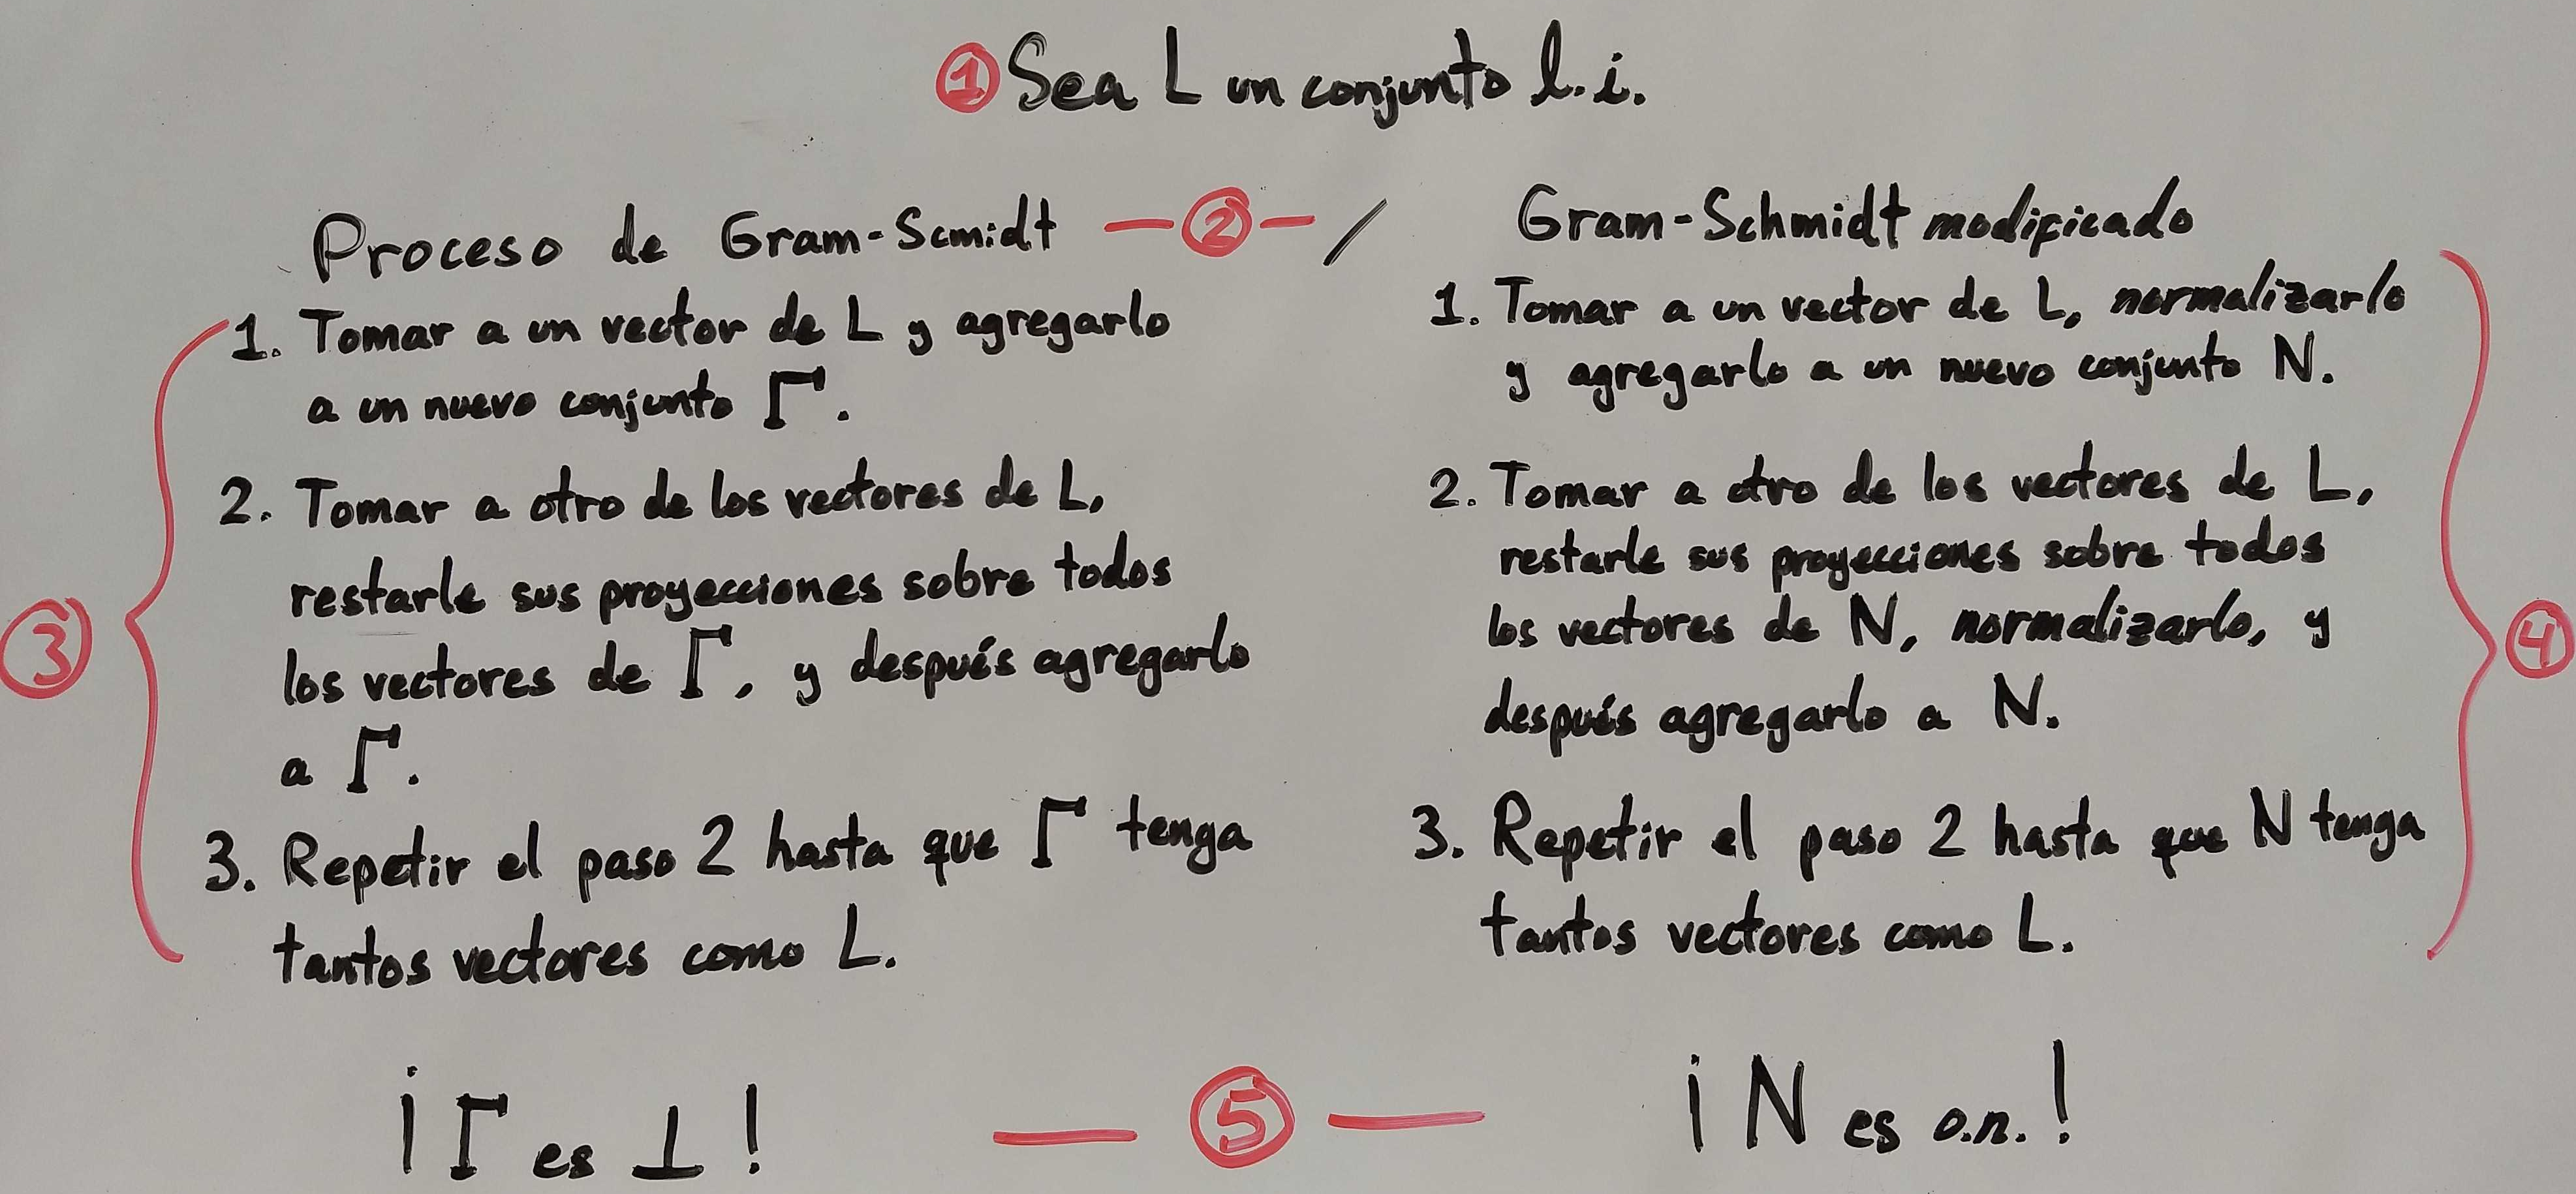
\includegraphics[width=17cm]{Ortogonalizacion_y_ortonormalizacion-1.png}
\end{figure}

En espacios vectoriales de dimensión finita, ambos procesos siempre se pueden aplicar para obtener una base ortogonal u ortonormal del espacio a partir de cualquier base arbitraria. Esto se conoce como el Teorema de Gram-Schmidt. Las bases ortogonales y ortonormales tienen aplicaciones sumamente importantes, como veremos durante el resto de la serie de videos\footnote{Mejor porner los vectores ``n''s con gorritos ya que, por la forma en que los estamos definiendo, son unitarios, y el objetivo es que la base $N$ sea ortonormal.}.

\begin{figure}[h!]
    \centering
    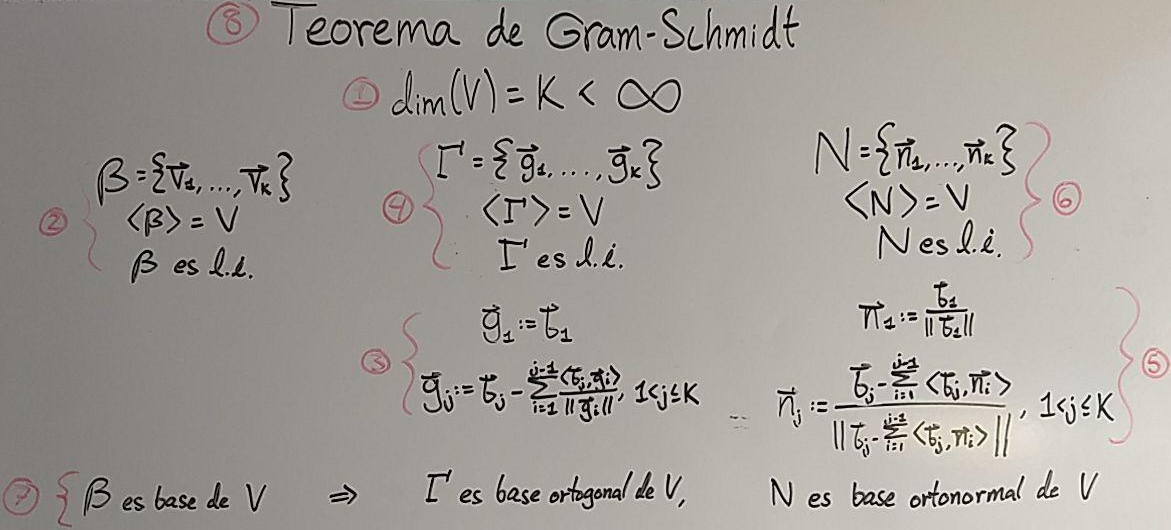
\includegraphics[width=17cm]{Ortogonalizacion_y_ortonormalizacion-2.png}
\end{figure}

\newpage
\section{Escena final}

\begin{center}
    Sea $V$ un espacio vectorial con producto escalar.
\end{center}

Ejercicio 2.1: Demuestra que
\begin{align*}
    \bigg\langle \bigg\{\vec{u}, \vec{v} - \frac{\langle \vec{v}, \vec{u}\rangle}{||\vec{u}||}\hat{u} \bigg\}\bigg\rangle = \langle \{\vec{u},\vec{v}\} \rangle
\end{align*} para $\vec{u},\vec{v}\in V$ con $\vec{u},\vec{v}\neq\vec{0}$ y dibuja un ejemplo en $\mathbb{R}^2$.

\vspace{5mm}

Ejercicio 2.2: Demuestra que cualquier conjunto ortogonal de vectores no nulos es linealmente independiente.

\vspace{5mm}

Pregunta 2.1: ¿Qué sucedería si aplicáramos el proceso de Gram-Schmidt a un conjunto de vectores linealmente \emph{dependiente}?

Pregunta 2.2: ¿Qué sucedería si, en el proceso de Gram-Schmidt modificado, normalizáramos a alguno de los vectores \emph{antes} de ortogonalizarlo en vez de  \emph{después}?

\end{document}